% !TEX root = paper.tex

\section {Results}
\label{sec:results}

\begin{figure}[!hbt]
	\centering
	\subfigure{ 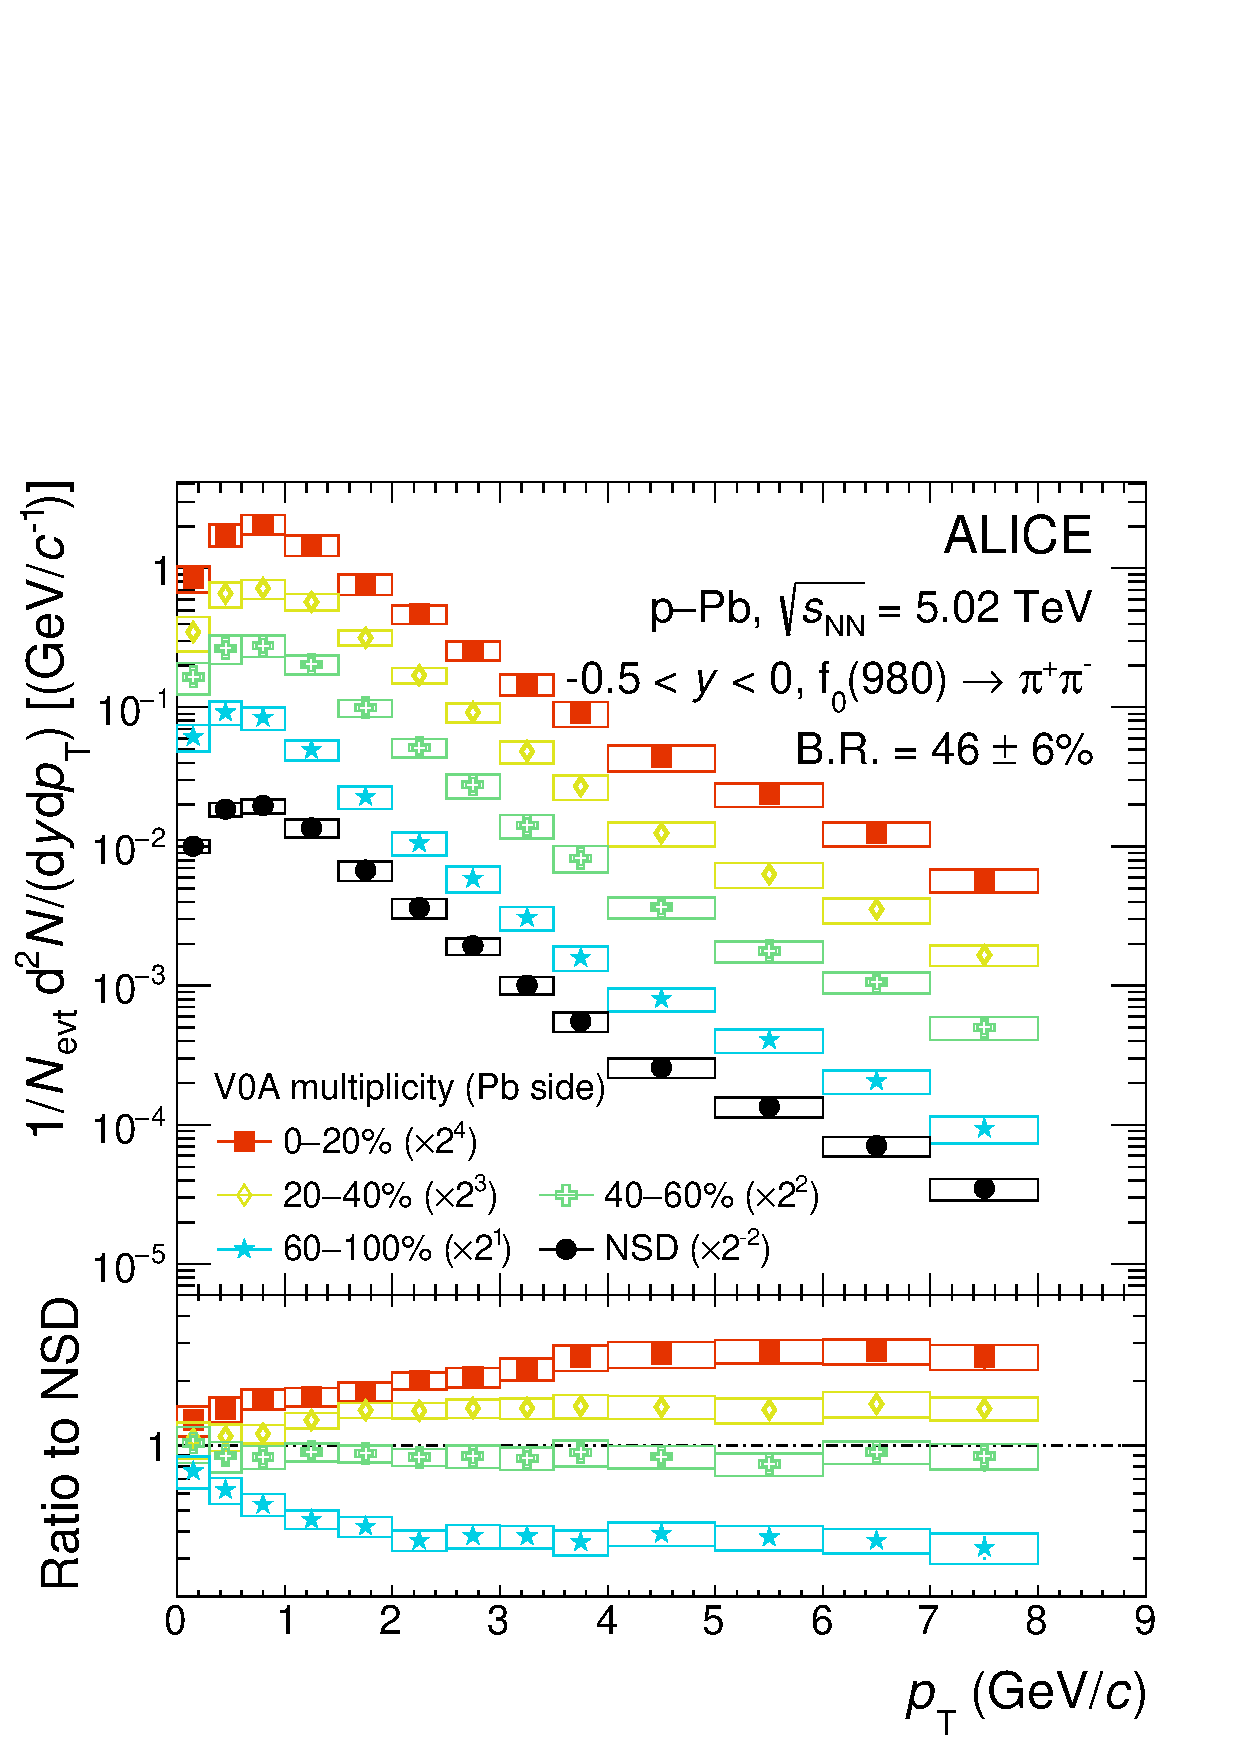
\includegraphics[width=0.6 \textwidth]{figures/Fig2_pt_all.pdf} }
	\caption{ Transverse momentum spectra of \fzero~in p--Pb collisions at \snn~=~5.02~TeV for different multiplicity classes, which are scaled for visibility. Statistical and systematic uncertainties are shown as error bars and boxes, respectively. The lower panel shows the ratios of the specific spectra to the minimum-bias NSD spectrum. }
	\label{fig:pt}
\end{figure}

Figure~\ref{fig:pt} shows the $p_{\mathrm{T}}$ spectra of \fzero~in p--Pb collisions at \snn~=~5.02~TeV measured in the range of 0~$<p_{\mathrm{T}}<$~8~GeV/$c$ for different multiplicity classes. Each spectrum is scaled with the number denoted in the figure for visibility. The lower panel of Fig.~\ref{fig:pt} shows the ratios of each $p_{\mathrm{T}}$ spectrum to the minimum-bias $p_{\mathrm{T}}$ spectrum. Increasing mean $p_{\mathrm{T}}$ are observed with the increasing multiplicity.

\begin{figure}[!hbt]
	\centering
	\subfigure{ 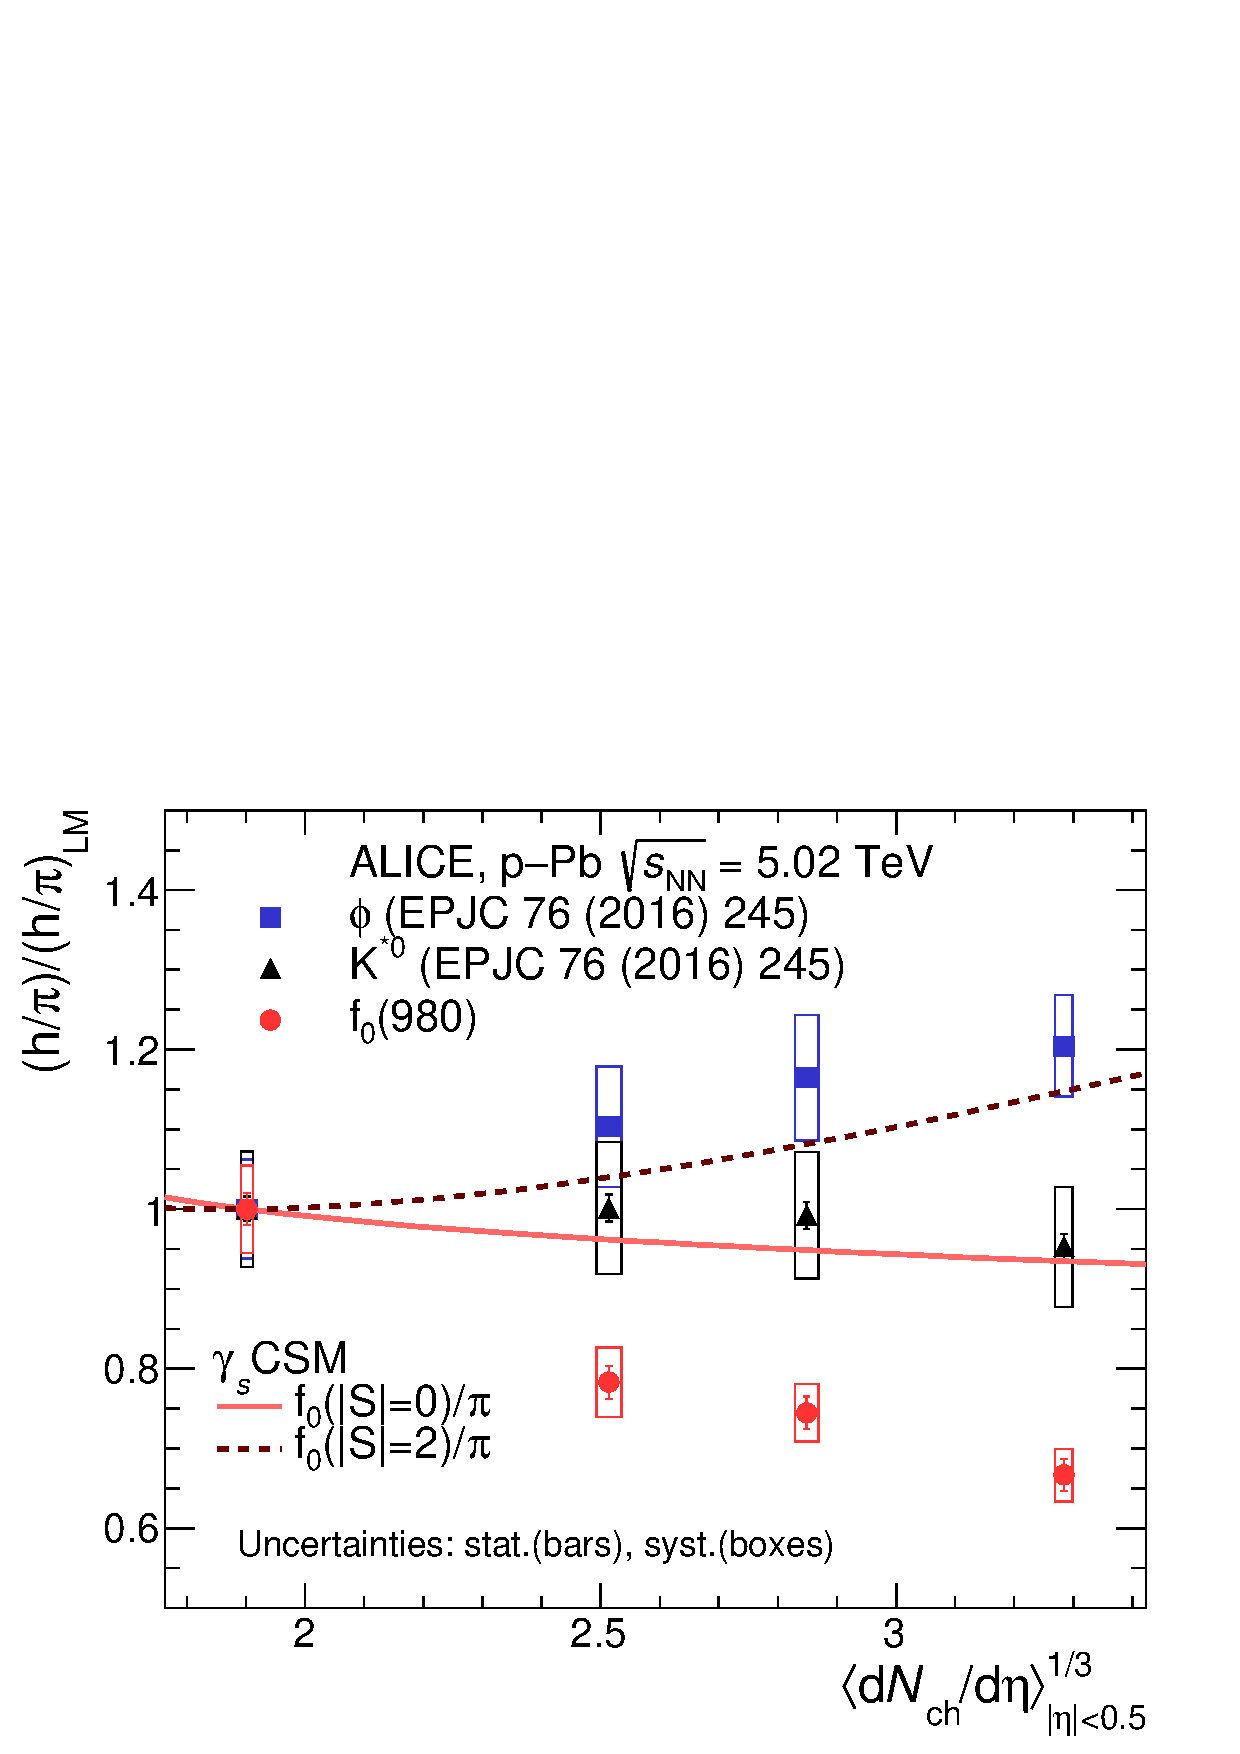
\includegraphics[width=0.6 \textwidth]{figures/Fig4_dr_pion_addCSM.pdf} }
	\caption{ Double ratio of $\phi$, $\rm{}K^{*0}$(892), and \fzero~to $\pi$ as a function of charged-particle multiplicity elevated to 1/3. The ratios are divided by the ratio in low-multiplicity events to make the first point unity. Predictions from Canonical statistical model are represented with solid lines. }
	\label{fig:f0piAddCSM}
\end{figure}

Figure~\ref{fig:f0piAddCSM} shows the double ratios of different particles to charged pion yields as a function of charged-particle multiplicity elevated to 1/3 in p--Pb collisions at \snn~=~5.02~TeV. The ratio of $\phi$ to $\pi$ is increasing with the multiplicity, which favors the observation of the strangeness enhancement~\cite{ALICE:2016fzo}. The ratio of $\rm{}K^{*0}$ to $\pi$ is flat with the increasing multiplicity even $\rm{}K^{*0}$ includes one strange quark. The flat trend is due to the two competing effects, the strangeness enhancement and rescattering effects, as the lifetime of $\rm{}K^{*0}$ is 4.2~fm/$c$~\cite{ParticleDataGroup:2020ssz}. The ratio of \fzero~to $\pi$ is decreasing as the multiplicity increases because of the short lifetime of \fzero, which suggests non-negative rescattering effects for \fzero. Predictions of the ratio of \fzero~to $\pi$ are shown in lines for different hidden strangeness assumptions for \fzero~by Canonical Statistical Model (CSM)~\cite{Vovchenko:2019kes}. The CSM with two hidden strangeness estimates the ratio to be increasing, which is opposite trend of the experimental result. Moreover, the CSM with zero hidden strangeness estimates the ratio to be flat, which also overestimates the data. The overestimation is attributed to no recattering effects in the CSM.

\begin{figure}[!hbt]
	\centering
	\subfigure{ 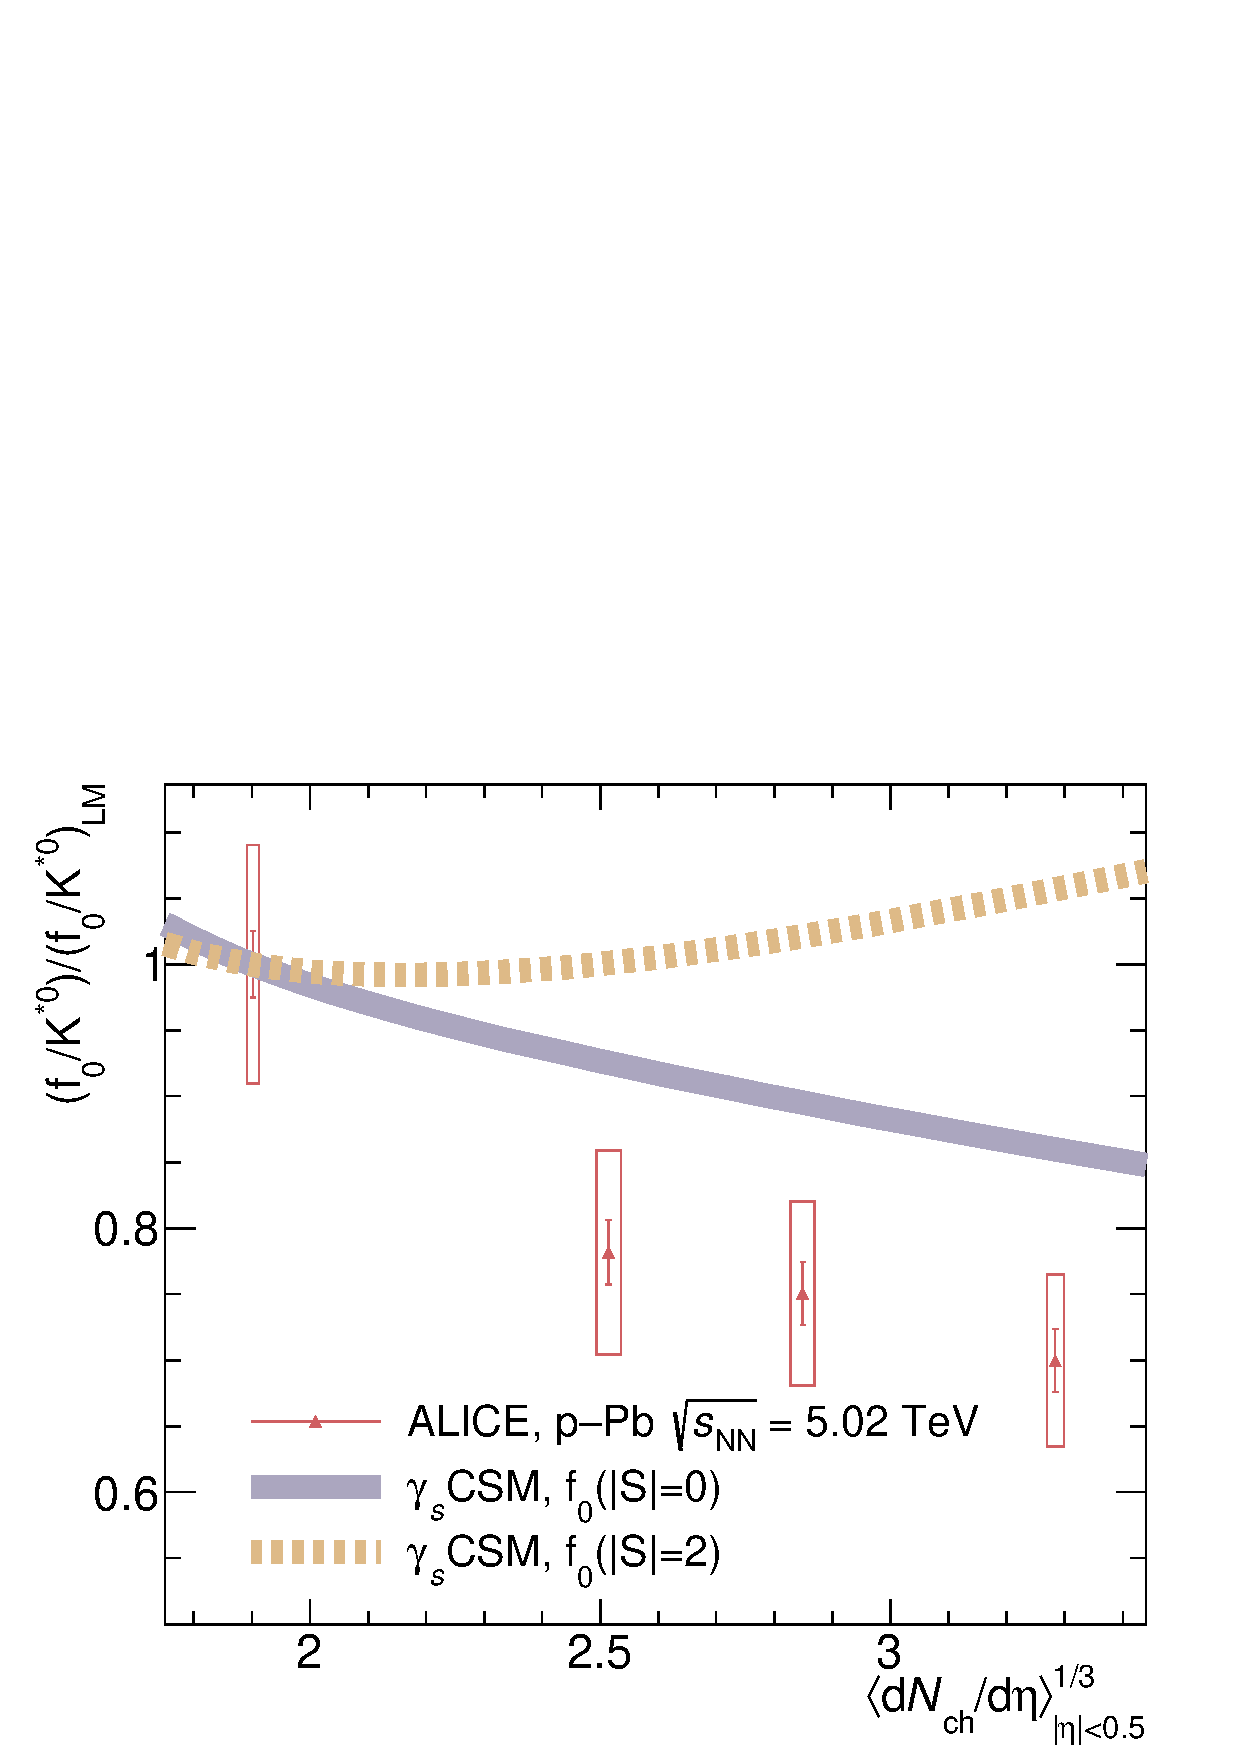
\includegraphics[width=0.6 \textwidth]{figures/Fig4_dr_kstar_addCSM.pdf} }
	\caption{ Double ratio of \fzero~to $\rm{}K^{*0}$ yields as a function of charged-particle multiplicity elevated to 1/3. The ratios are divided by the ratio in low-multiplicity events to make the first point unity. Predictions from Canonical statistical model are represented with solid lines. }
	\label{fig:f0KSAddCSM}
\end{figure}

Figure~\ref{fig:f0KSAddCSM} shows the double ratio of \fzero~to $\rm{}K^{*0}$ yields as a function of charged-particle multiplicity elevated to 1/3 in p--Pb collisions at \snn~=~5.02~TeV and predictions from the CSM with different hidden strangeness assumptions. The ratio is decreasing with the increasing multiplicity, and this trend is qualitatively described with the zero hidden strangeness assumption. The lifetimes of \fzero~and $\rm{}K^{*0}$ are estimated to be comparable, indicating that rescattering effects would not be much different. Hence, the decreasing trend of the ratio is weakly affected by rescattering effects. The CSM prediction with two hidden strangeness assumption is mildly increasing as the multiplicity increases, which is also opposite to the experimental result. Therefore, decreasing trend of the ratio of \fzero~to $\rm{}K^{*0}$ can suggest absence of the strange quark in \fzero.

\begin{figure}[!hbt]
	\centering
	\subfigure{ 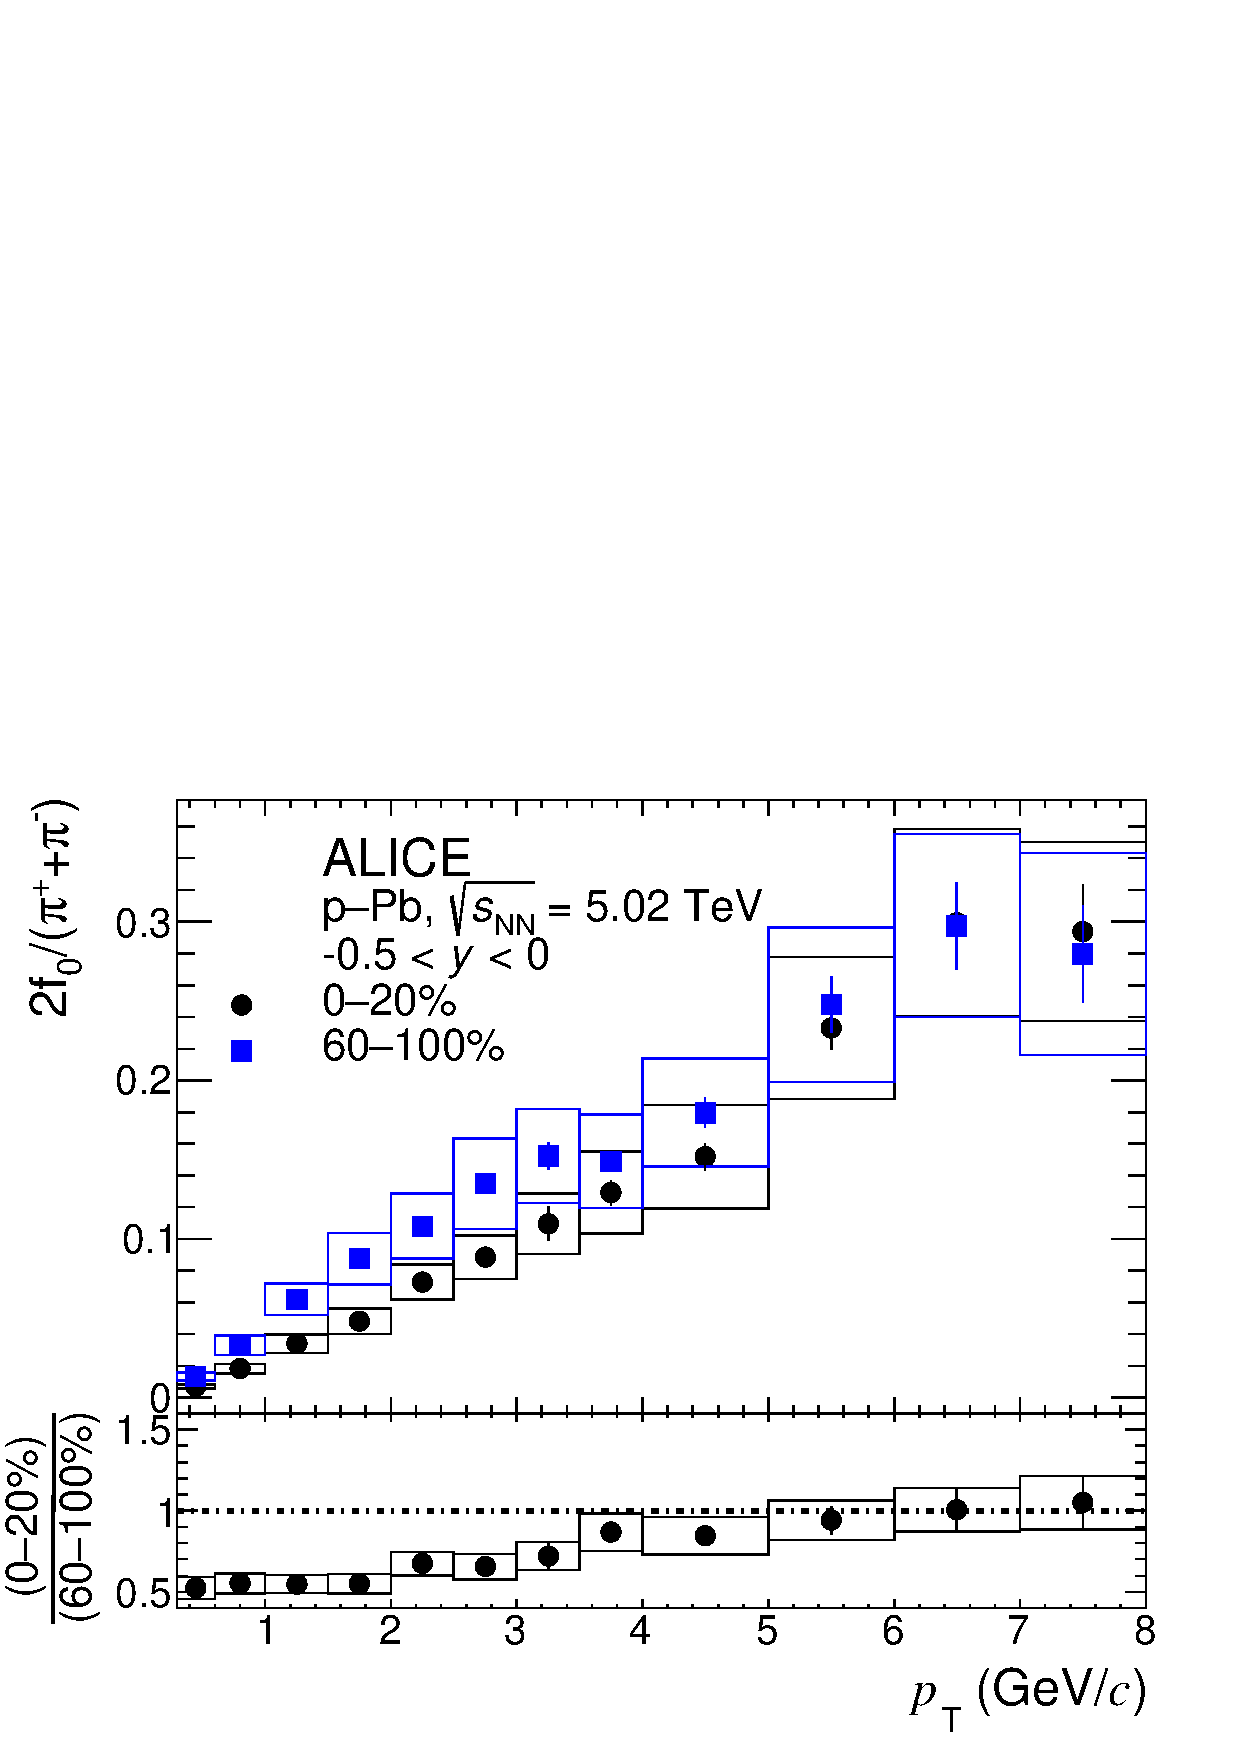
\includegraphics[width=0.6 \textwidth]{figures/Fig5_DR_pt_pion.pdf} }
	\caption{ Particle yield ratio of \fzero~to $\pi$ as a function of $p_{\rm{T}}$ in high-multiplicity (circles) and low-multiplicity (triangles) p--Pb collisions at \snn~5.02~TeV. The lower panel shows the double ratio of high-multiplicity to low-multiplicity \fzero/$\pi$. }
	\label{fig:f0piPt}
\end{figure}

Figure~\ref{fig:f0piPt} shows $p_{\mathrm{T}}$-differential particle yield ratio of \fzero~to $\pi$ in high-multiplicity (HM) and low-multiplicity (LM) p--Pb collisions at \snn~=~5.02~TeV. The ratios are consistent within one sigma for $p_{\mathrm{T}}>$~4~GeV/$c$, while the double ratio of HM to LM is suppressed at low $p_{\mathrm{T}}$, which is shown in the lower panel of Fig.~\ref{fig:f0piPt}. The $p_{\mathrm{T}}$ dependence of the double ratio indicates that the suppression of the integrated yield is a low-$p_{\mathrm{T}}$ effect, which is the qualitatively same $p_{\mathrm{T}}$ dependence as the suppression of the $\rm{}K^{*0}/K$~\cite{ALICE:2019etb}.

\begin{figure}[!hbt]
	\centering
	\subfigure{ 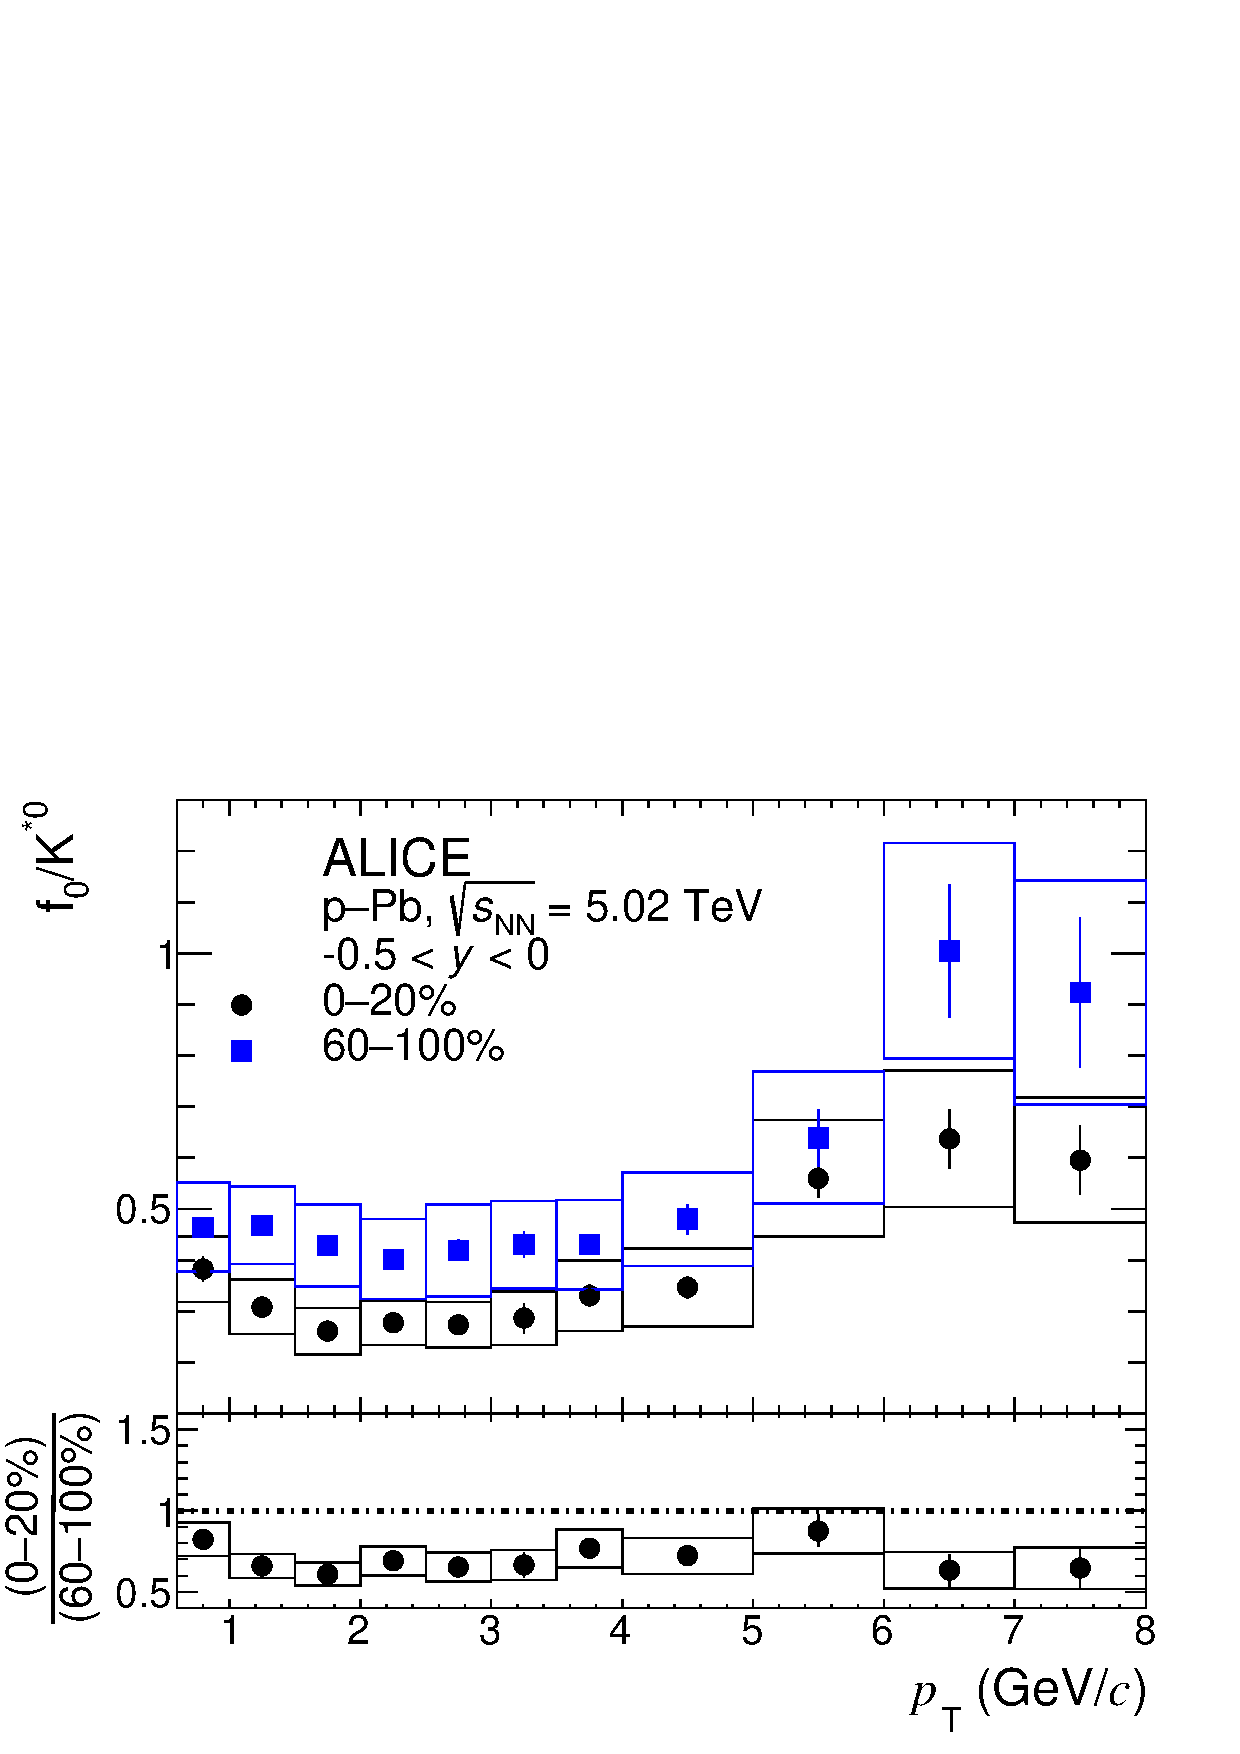
\includegraphics[width=0.6 \textwidth]{figures/Fig6_DR_pt_kstar.pdf} }
	\caption{ Particle yield ratio of \fzero~to $\rm{}K^{*0}$(892) as a function of $p_{\rm{T}}$ in high-multiplicity (circles) and low-multiplicity (triangles) p--Pb collisions at \snn~5.02~TeV. The lower panel shows the double ratio of high-multiplicity to low-multiplicity \fzero/$\rm{}K^{*0}$(892).  }
	\label{fig:f0KsPt}
\end{figure}

Figure~\ref{fig:f0KsPt} shows $p_{\mathrm{T}}$-differential particle yield ratio of \fzero~to $\rm{}K^{*0}$ in HM and LM p--Pb collisions at \snn~=~5.02~TeV. The ratio from HM events is suppressed in the measured entire $p_{\mathrm{T}}$ range, which is significantly different from the $p_{\mathrm{T}}$ dependence of $\rm{}K^{*0}/K$ or \fzero/$\pi$. The different $p_{\mathrm{T}}$ dependence of the double ratio indicates that the other effects, rather than rescattering effects, are present. For instance, the enhancement of $\rm{}K^{*0}$ yield due to the strangeness enhancement can explain the suppression at the entire $p_{\mathrm{T}}$ range. As a result, the relative suppression suggests no strange quark in \fzero.

\begin{figure}[!hbt]
	\centering
	\subfigure{ 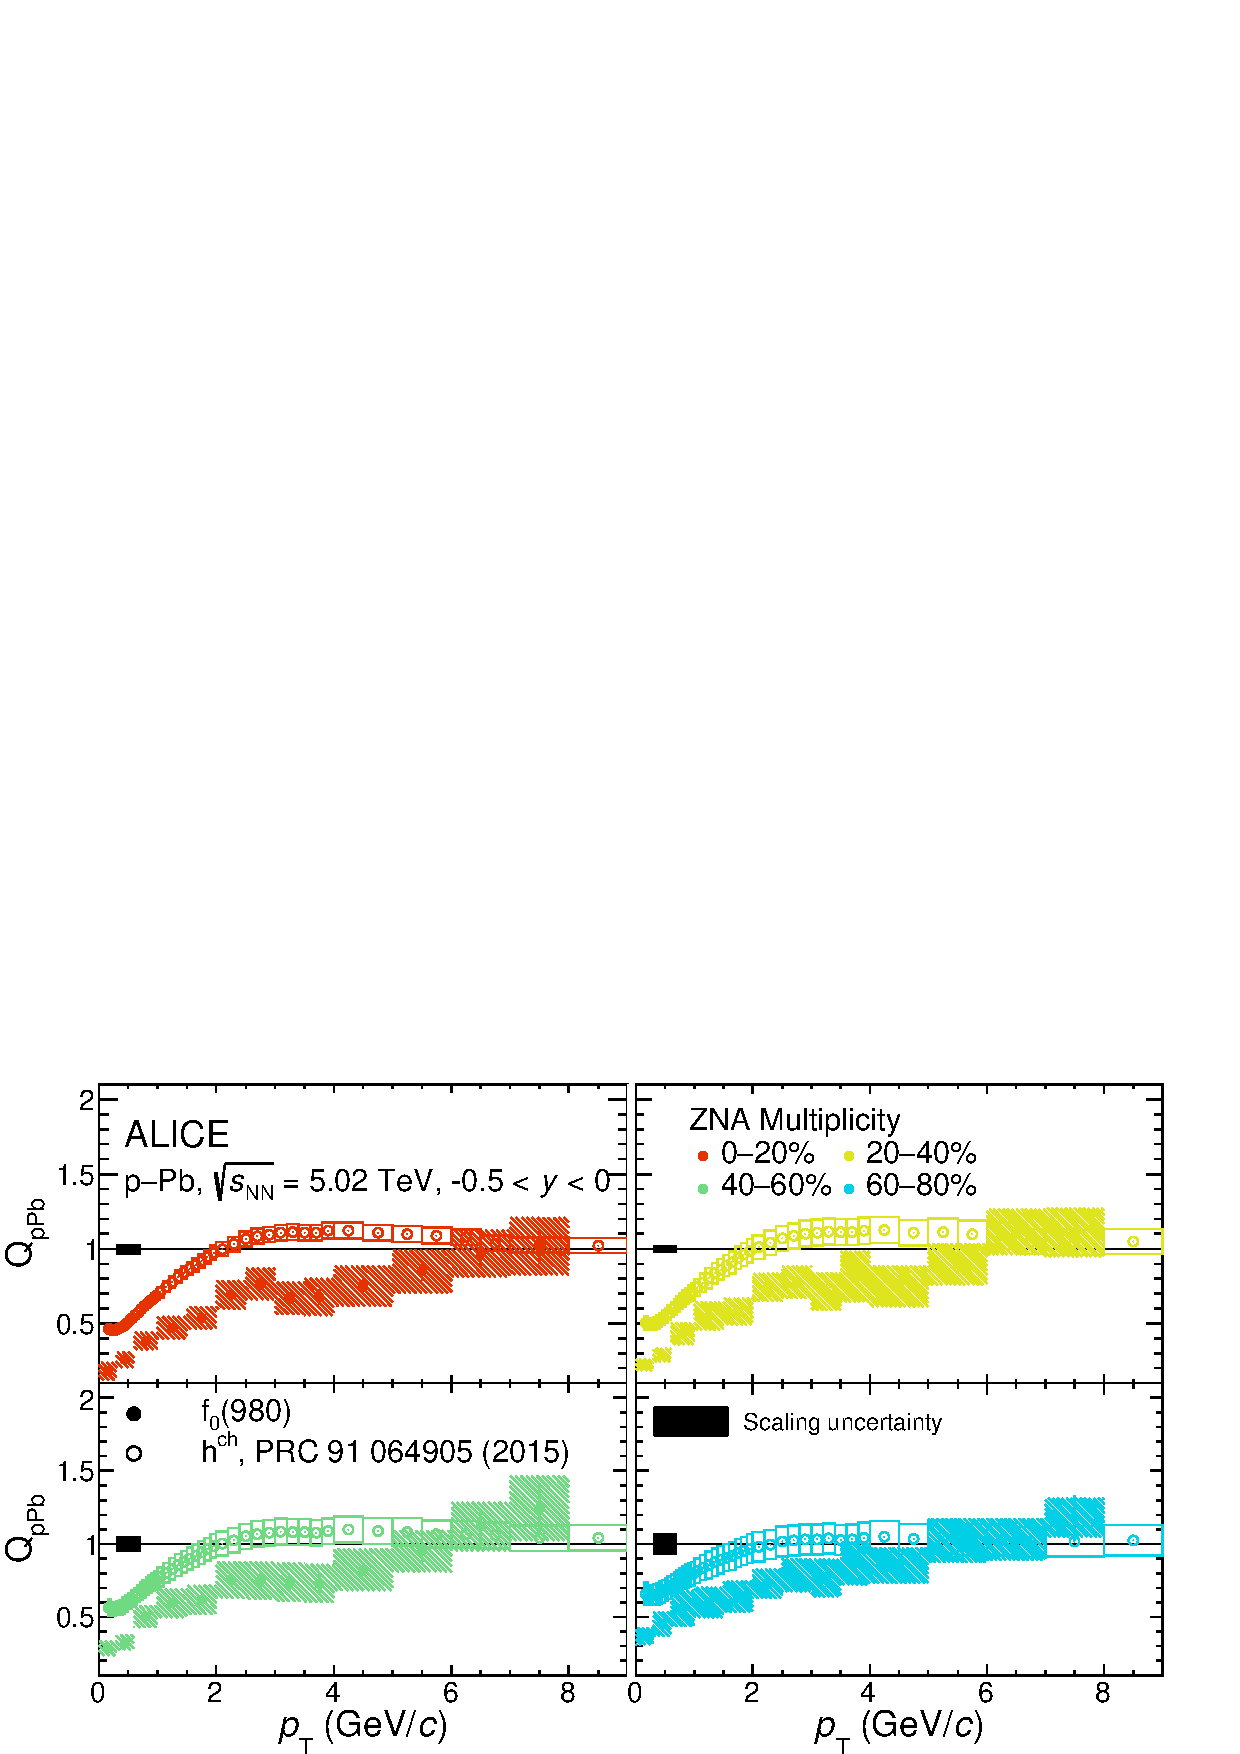
\includegraphics[width=0.8 \textwidth]{figures/Fig7_QpPb.pdf} }
	\caption{ Nuclear modification factor ($Q_{\rm{pPb}}$) of \fzero~as a function of $p_{\rm{T}}$ in p--Pb collisions at \snn~5.02~TeV for different multiplicity classes. Statistical and systematic uncertainties are shown as error bars and boxes, respectively. Open boxes around $p_{\rm{T}}$~=~0.5~GeV/$c$ represent the binary collision scaling uncertainties. The $Q_{\rm{pPb}}$ of \fzero~is compared with \fzero~of charged hadrons. }
	\label{fig:QpPb}
\end{figure}

Figure~\ref{fig:QpPb} shows the nuclear modification factor ($Q_{\rm{pPb}}$) of \fzero~in p--Pb collisions at \snn~=~5.02~TeV in different multiplicity classes. The systematic uncertainties are calculated with the assumption that there is no correlated uncertainty between the cross section in pp and p--Pb collisions. The \fzero~is much suppressed than charged hadrons in all measured centrality intervals for $p_{\mathrm{T}}<$~4~GeV/$c$. As $p_{\mathrm{T}}$ increases, the difference of $Q_{\rm{pPb}}$ gets smaller. The observation can be also related to the existence of rescattering effects for \fzero. In addition, the $Q_{\rm{pPb}}$ does not exhibit Cronin peak~\cite{Cronin:1974zm} at the intermediate $p_{\mathrm{T}}$ in HM events, while all baryons do. No Cronin peak for \fzero~might suggest the number of constituent quarks of \fzero~to be smaller than three.